\documentclass[14pt, unknownkeysallowed]{beamer}

\usepackage{tikz}
\usepackage{comment}
\usepackage{fancyvrb}
\usepackage{tikz}
\usetikzlibrary{arrows,decorations.pathmorphing,backgrounds,positioning,fit,petri}
\usepackage{circuitikz} % for circuits!
\usetikzlibrary{arrows.meta} % for loads
\usepackage{float}
\usepackage{listings}

\usepackage{hyperref}

\usepackage[default]{berasans}
\renewcommand*\familydefault{\sfdefault}  %% Only if the base font of the document is to be sans serif
\usepackage[T1]{fontenc}

\setbeamertemplate{navigation symbols}{}
\usetheme{Dresden}
\usecolortheme{seagull}
\usefonttheme{professionalfonts}


%\title{Long-Term Simulation of Power System Dynamics using Time Sequenced Power Flows}
\title{Long-Term Power System Dynamic Simulation using Time Sequenced Power-Flows}
\author{Thad Haines}
\institute[MT TECH]{Montana Tech - Master's Thesis Research Project}
\date{February 5th, 2019}

\newcounter{assumptions}

\begin{document}

\begin{frame}
\titlepage
\end{frame}

%************************************************
\section{Introduction}
%________________________________________________
\subsection{Overview of Project}
%------------------------------------------------
\begin{frame}
What are long-term dynamics (LTD)? \tiny[1] \vspace{-2em}\\
\begin{figure}
	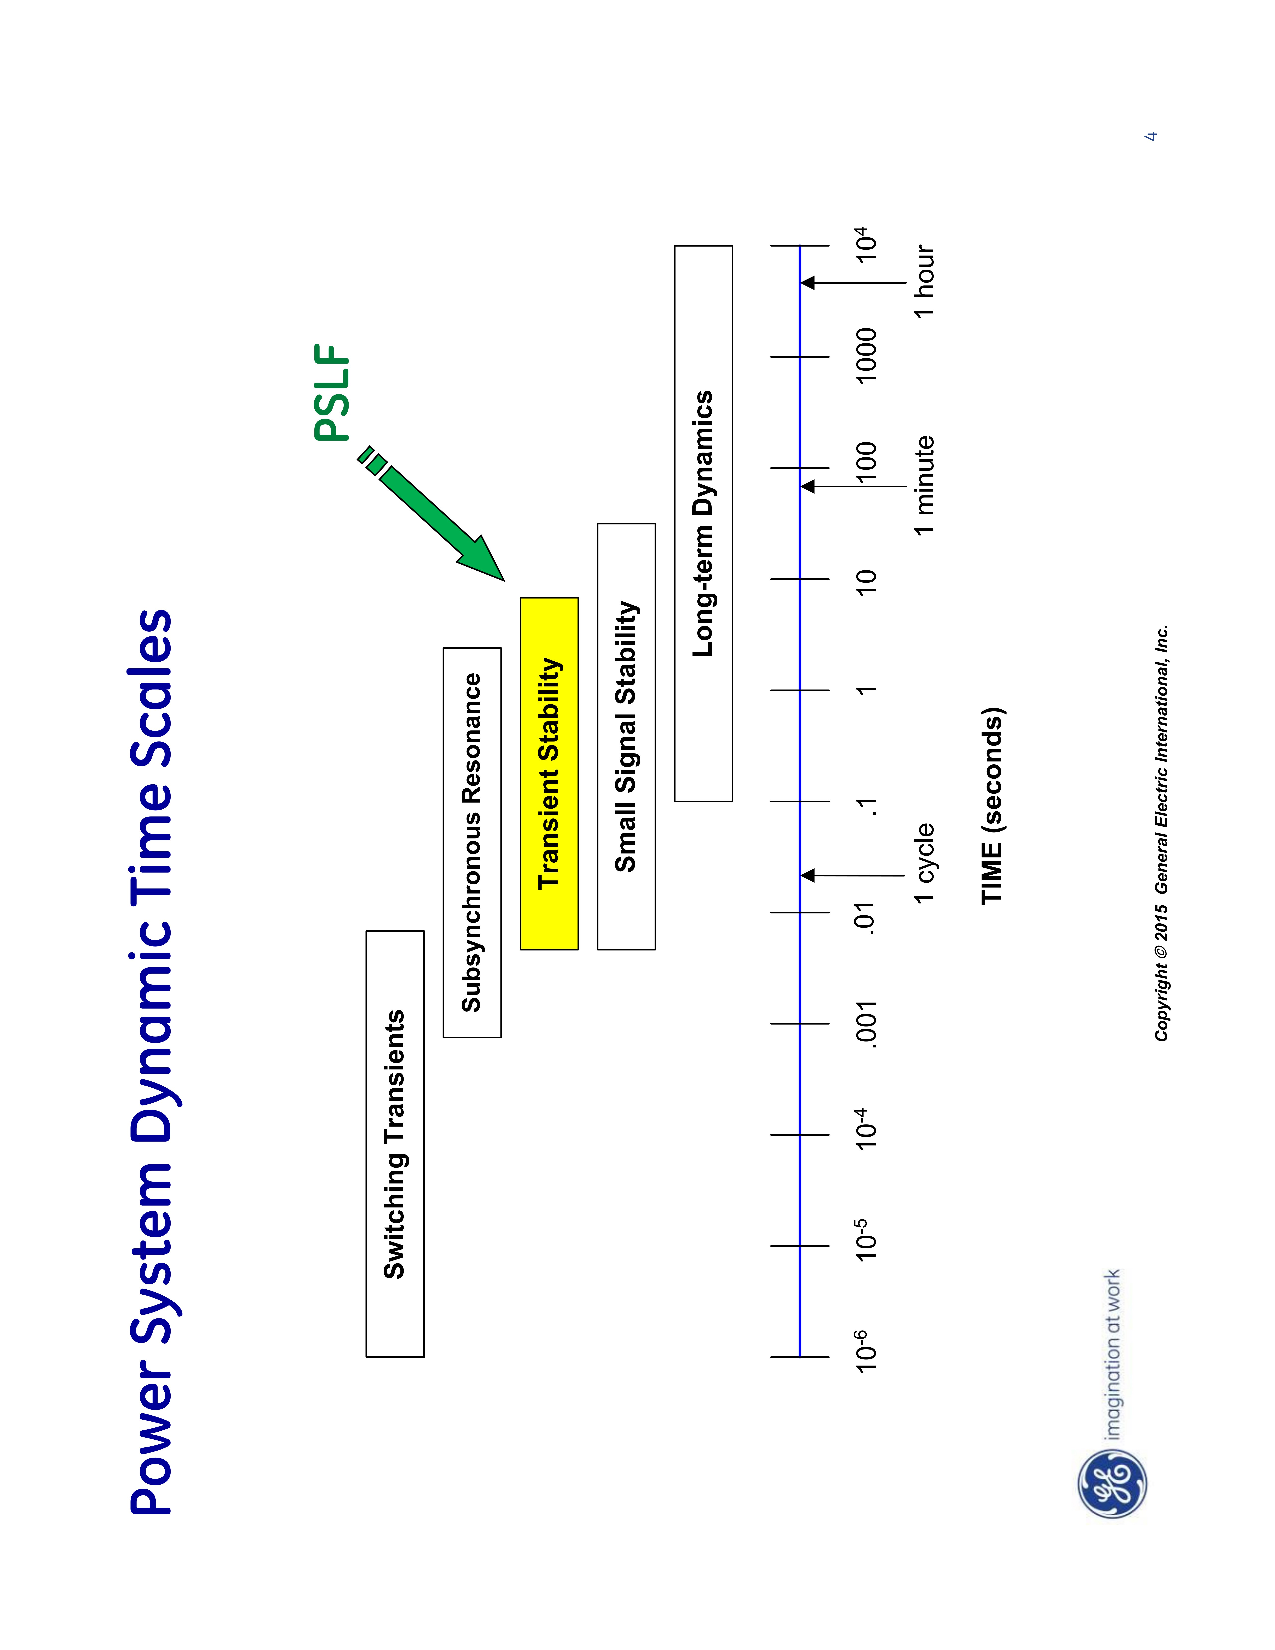
\includegraphics[angle=-90,origin=c,width=1.05\linewidth]{GEtimeScales} 
\end{figure}
\end{frame}
%------------------------------------------------
\begin{frame}
Project Goals:
\begin{itemize}
	\item Develop software for LTD simulations.
	\item Use PSLF:
	\begin{itemize}
		\item Systems ($.sav$ files)
		\item Dynamic data ($.dyd$ files)
		\item Power-flow solver
	\end{itemize}
	\item Create power system models compatible with LTD time steps.
	\item Investigate long-term events.
	\begin{itemize}
		\item AGC
		\item Wind ramps
	\end{itemize}
\end{itemize}
\end{frame}
%------------------------------------------------

%************************************************
\section{Simulation Model}
%________________________________________________
\subsection{Assumptions, Coding Decisions, Approaches, and Software Operation.}
%------------------------------------------------
\begin{frame}
This simulation assumes:
\begin{enumerate}
\item Time steps of 0.5 to 1 second.
\item Fast dynamics are 'mostly' ignored.
\item System remains synchronized.
\item System frequency is described by the combined PU swing equation:
\setcounter{assumptions}{\value{enumi}} % allow for break in counting
\end{enumerate}
\[ \dot{\omega}_{sys} = \dfrac{1}{2H_{sys} } \left( \dfrac{P_{acc, sys} }{\omega_{sys}(t)} - D_{sys}\Delta\omega_{sys}(t)  \right)\] 
\begin{enumerate}
\setcounter{enumi}{\value{assumptions}}
\item No system damping $(D_{sys} = 0)$.
\end{enumerate}
\end{frame}
%------------------------------------------------

\begin{frame}
Python will be used because:
\begin{itemize}
	\item PSLF communication
	\item Free
	\item Community Libraries
	\item Object Oriented Programming (Agent-Based Modeling)
\end{itemize}
\end{frame}
%------------------------------------------------
\begin{frame}
\begin{itemize}
	\item Agent\\ An autonomous individual object with properties and methods in a computer simulation.
	\item Agent-Based Modeling\\ The idea that a system can be modeled using agents in an environment, and a description of agent-agent and agent-environment interactions. \tiny[2]
\end{itemize}
\end{frame}
%------------------------------------------------
\begin{frame}
\vspace{-.75em}
\begin{figure}
	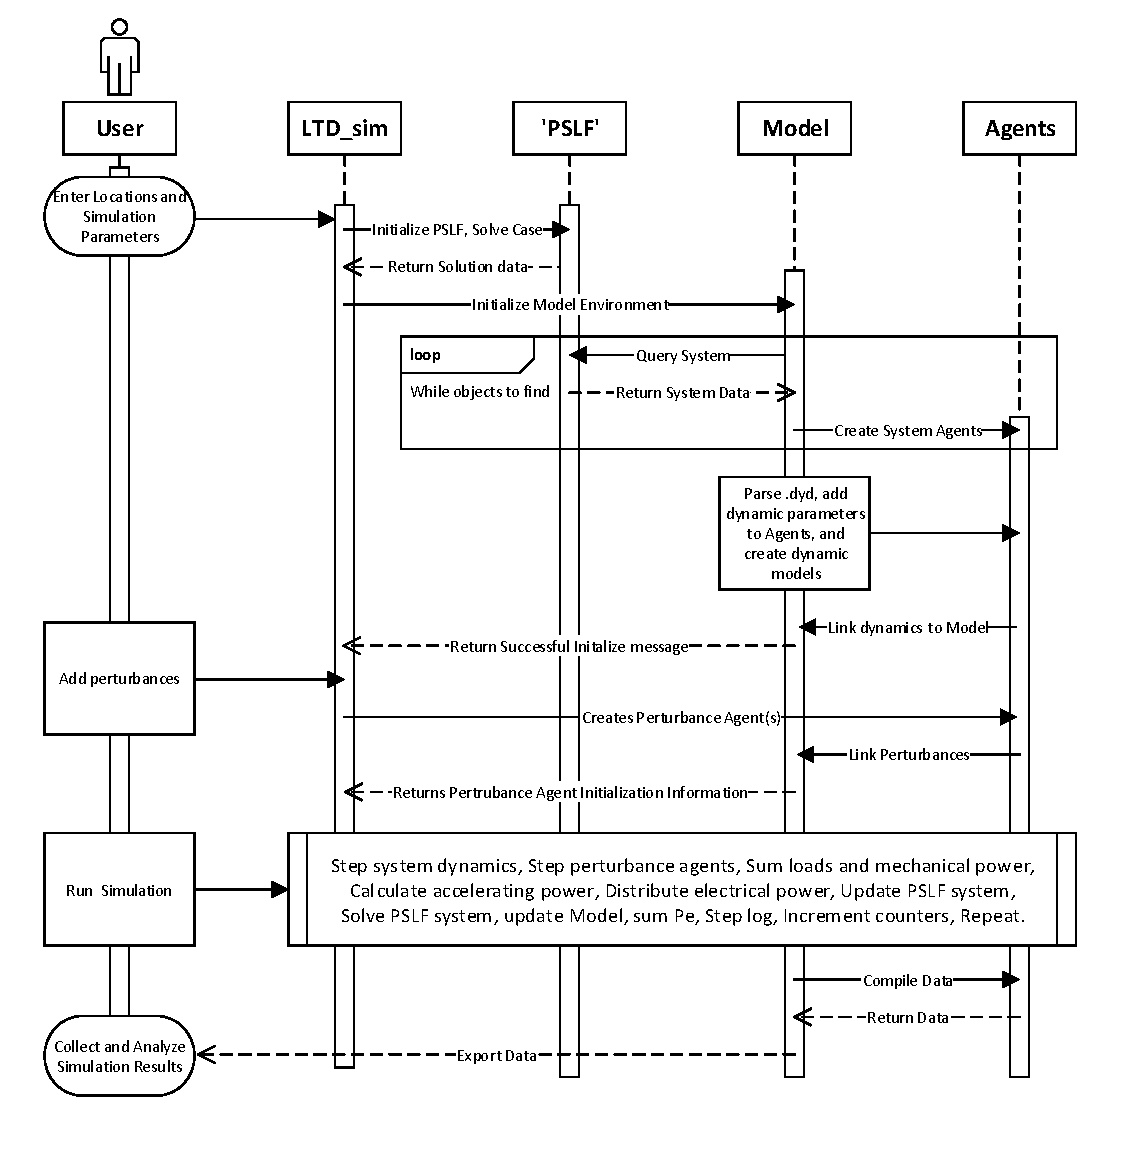
\includegraphics[height=1.07\textheight]{systemInit01.pdf}
\end{figure}
\end{frame}
%------------------------------------------------

%************************************************
\section{EE554 System}
%________________________________________________
\subsection{System Used for Initial Frequency Validation and Proof of Concept.}
%------------------------------------------------
\begin{frame}
EE554.sav test system:
\vspace{-1em}\\
\begin{figure}
	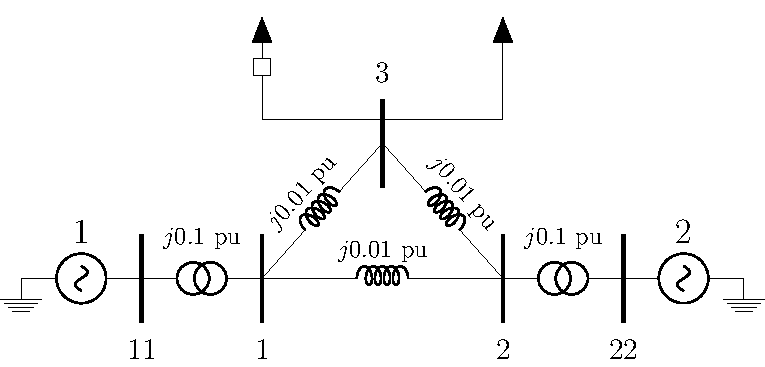
\includegraphics[width=\linewidth]{cicuitEE554}
\end{figure}
\vspace{-1em}
Generators are identical. \\PSLF models have exciters.
\end{frame}
%------------------------------------------------

%************************************************
\section{Initial Frequency Validation}
%________________________________________________
\subsection{+20 MW Load Step at t=2}
%------------------------------------------------
\begin{frame}
System Response
\begin{figure}
	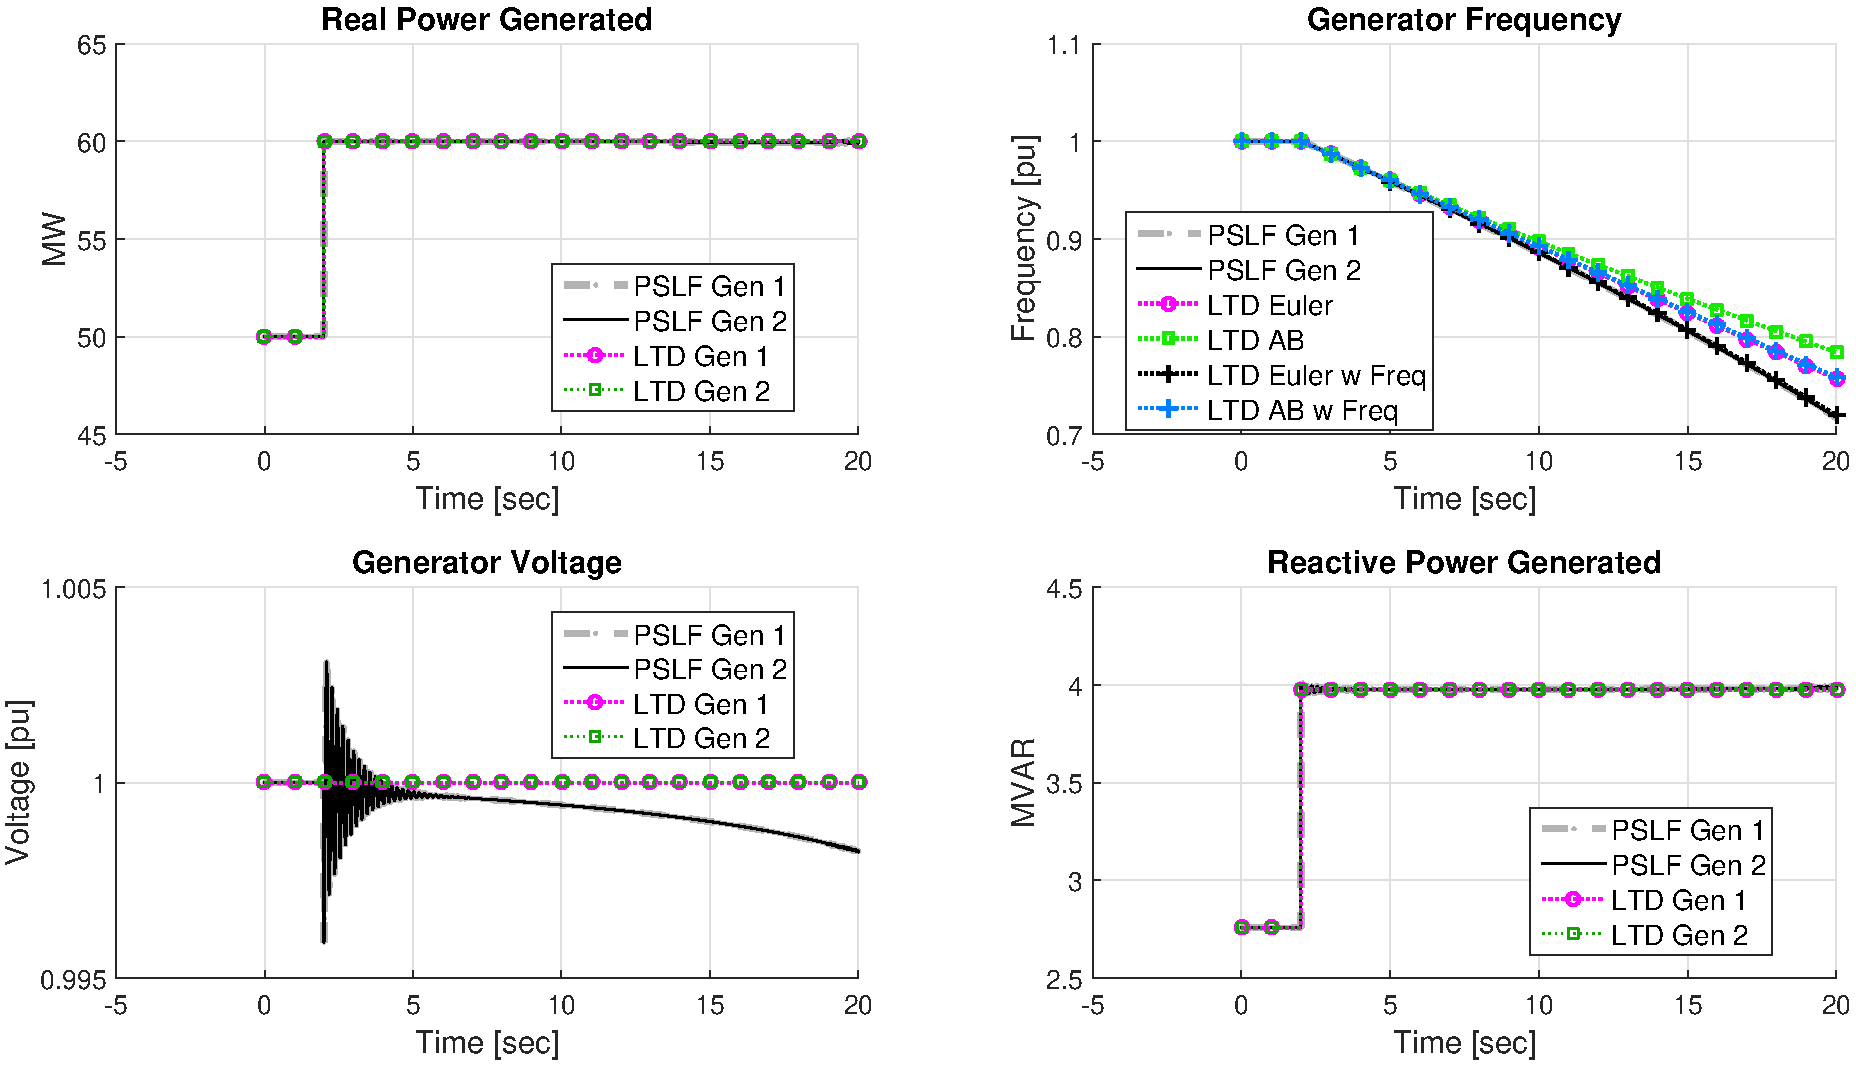
\includegraphics[width=\linewidth]{noGovExcLoadStepUpsys}
\end{figure}
\end{frame}
%------------------------------------------------
\begin{frame}
Detailed Frequency Response
\begin{figure}
	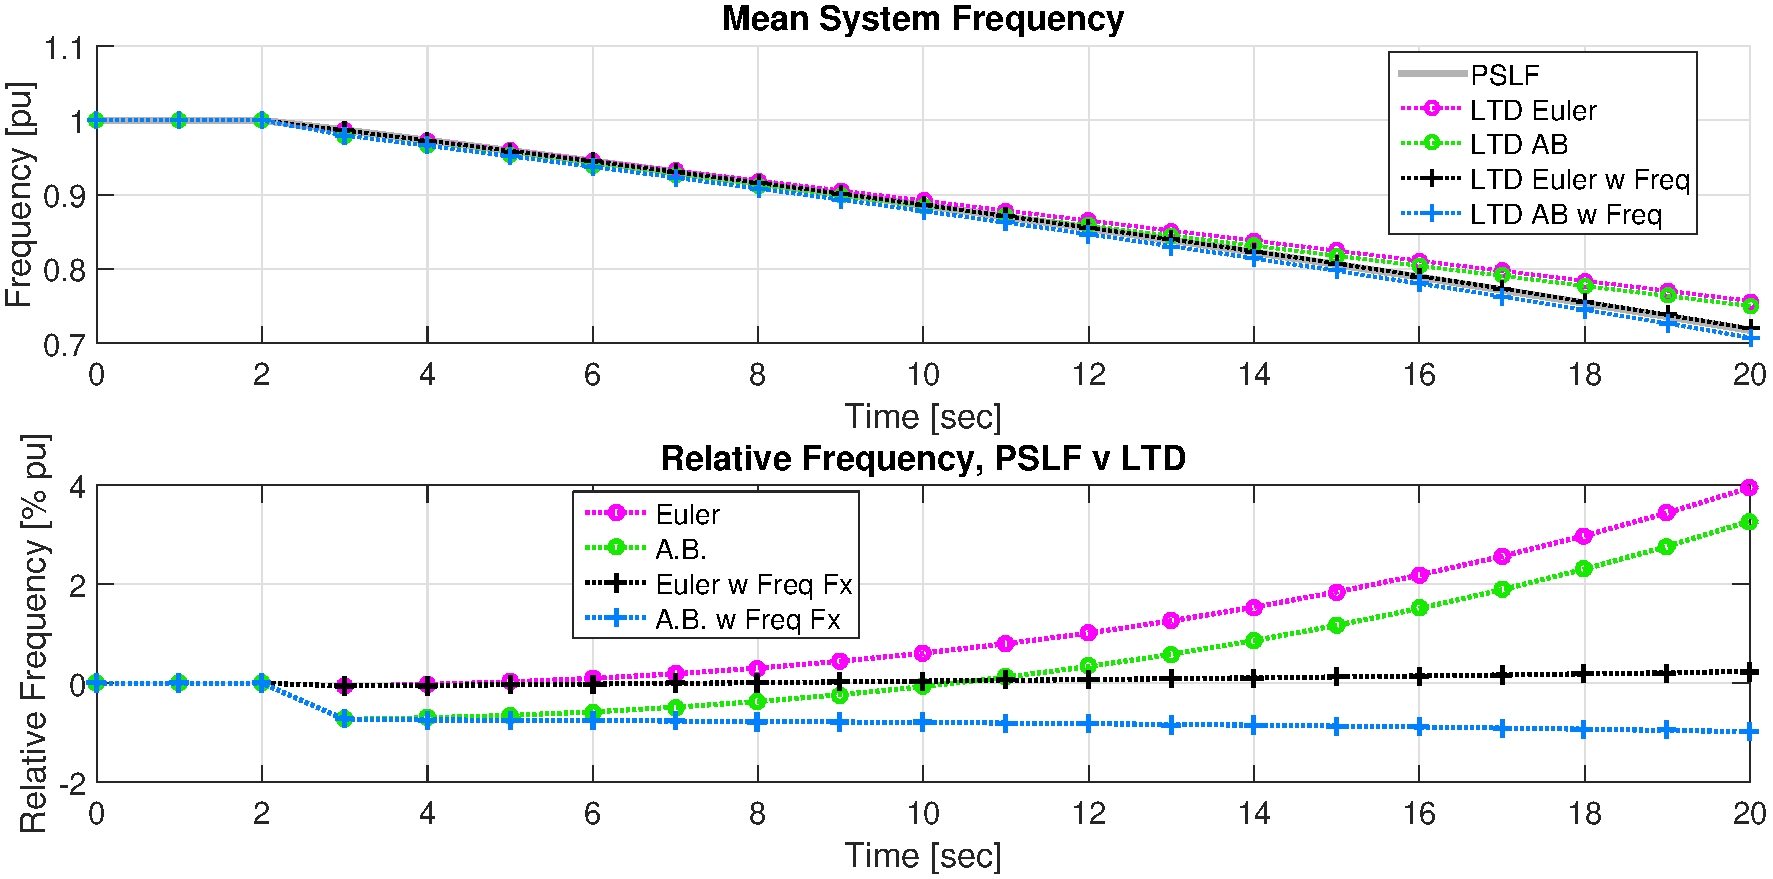
\includegraphics[width=\linewidth]{noGovExcLoadStepUpfreq}
\end{figure}
\end{frame}

%________________________________________________
\subsection{-20 MW Load Step at t=2}
%------------------------------------------------
\begin{frame}
System Response
\begin{figure}
	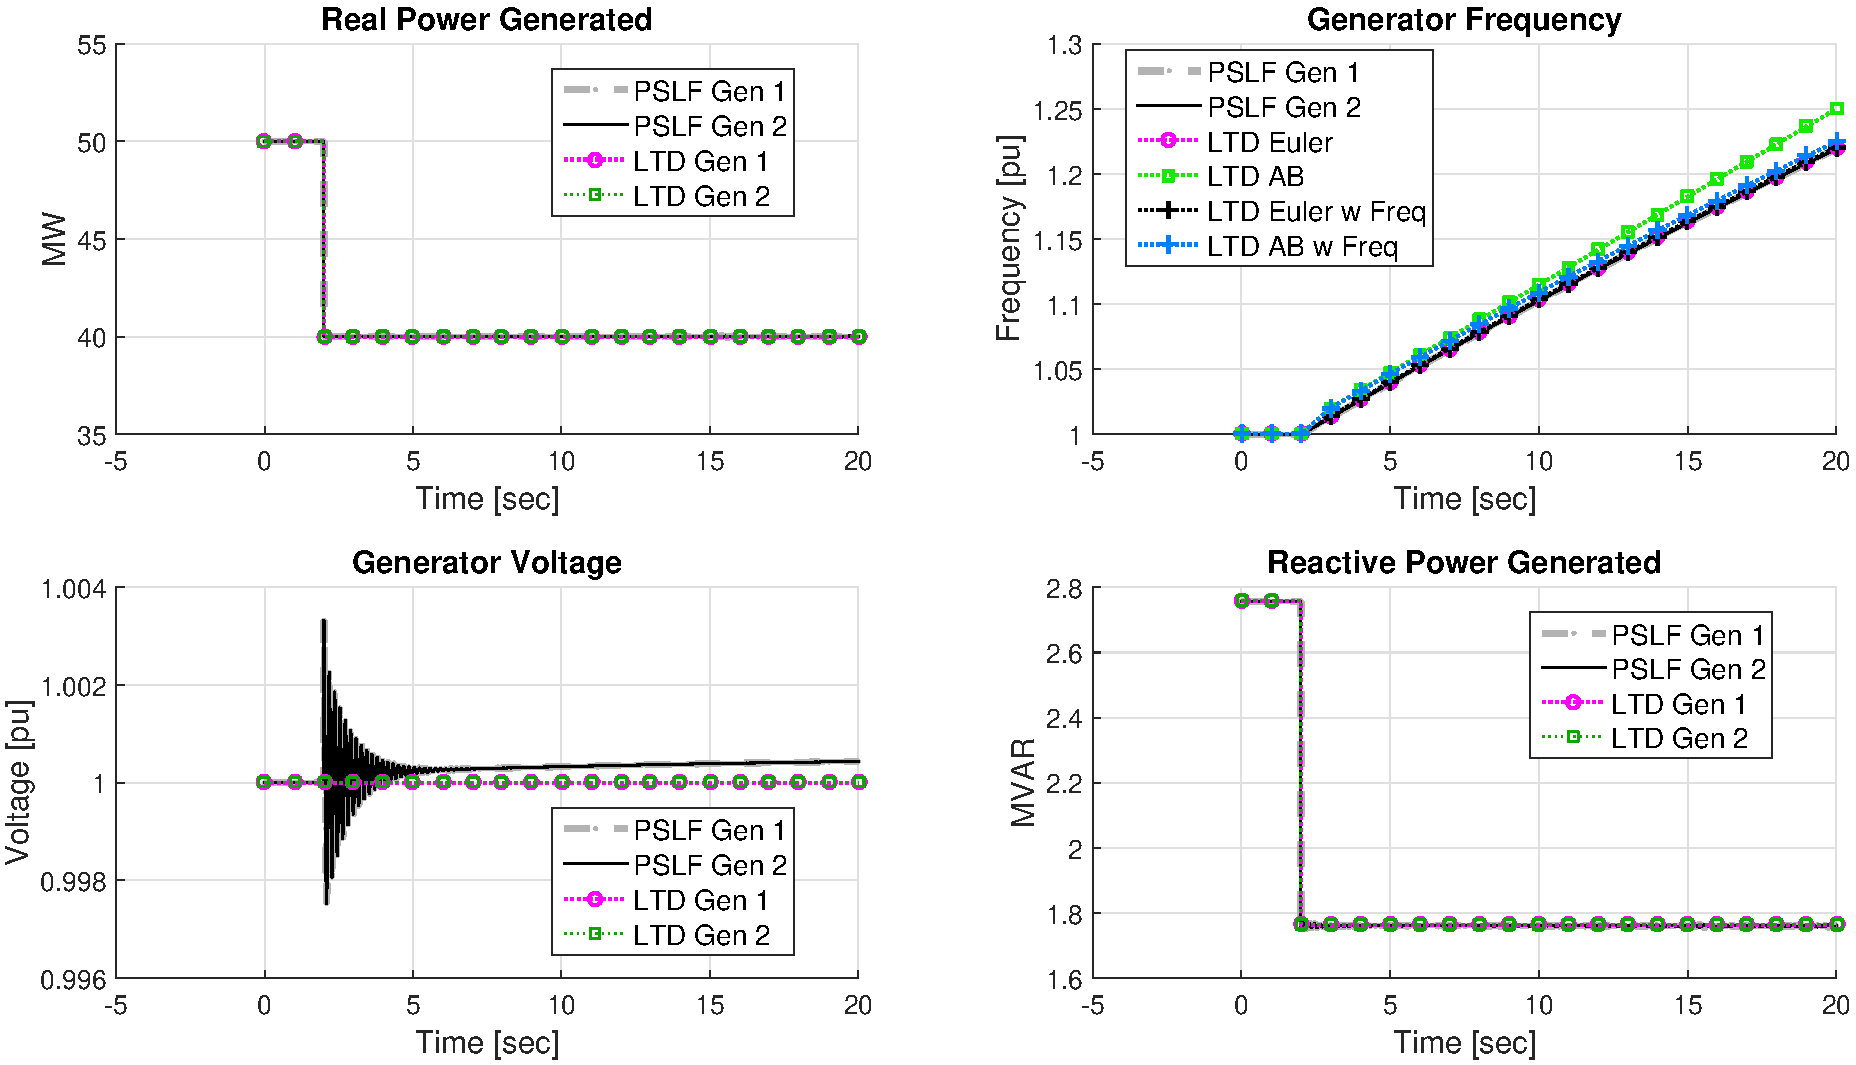
\includegraphics[width=\linewidth]{noGovExcLoadStepDsys}
\end{figure}
\end{frame}
%------------------------------------------------
\begin{frame}
Detailed Frequency Response
\begin{figure}
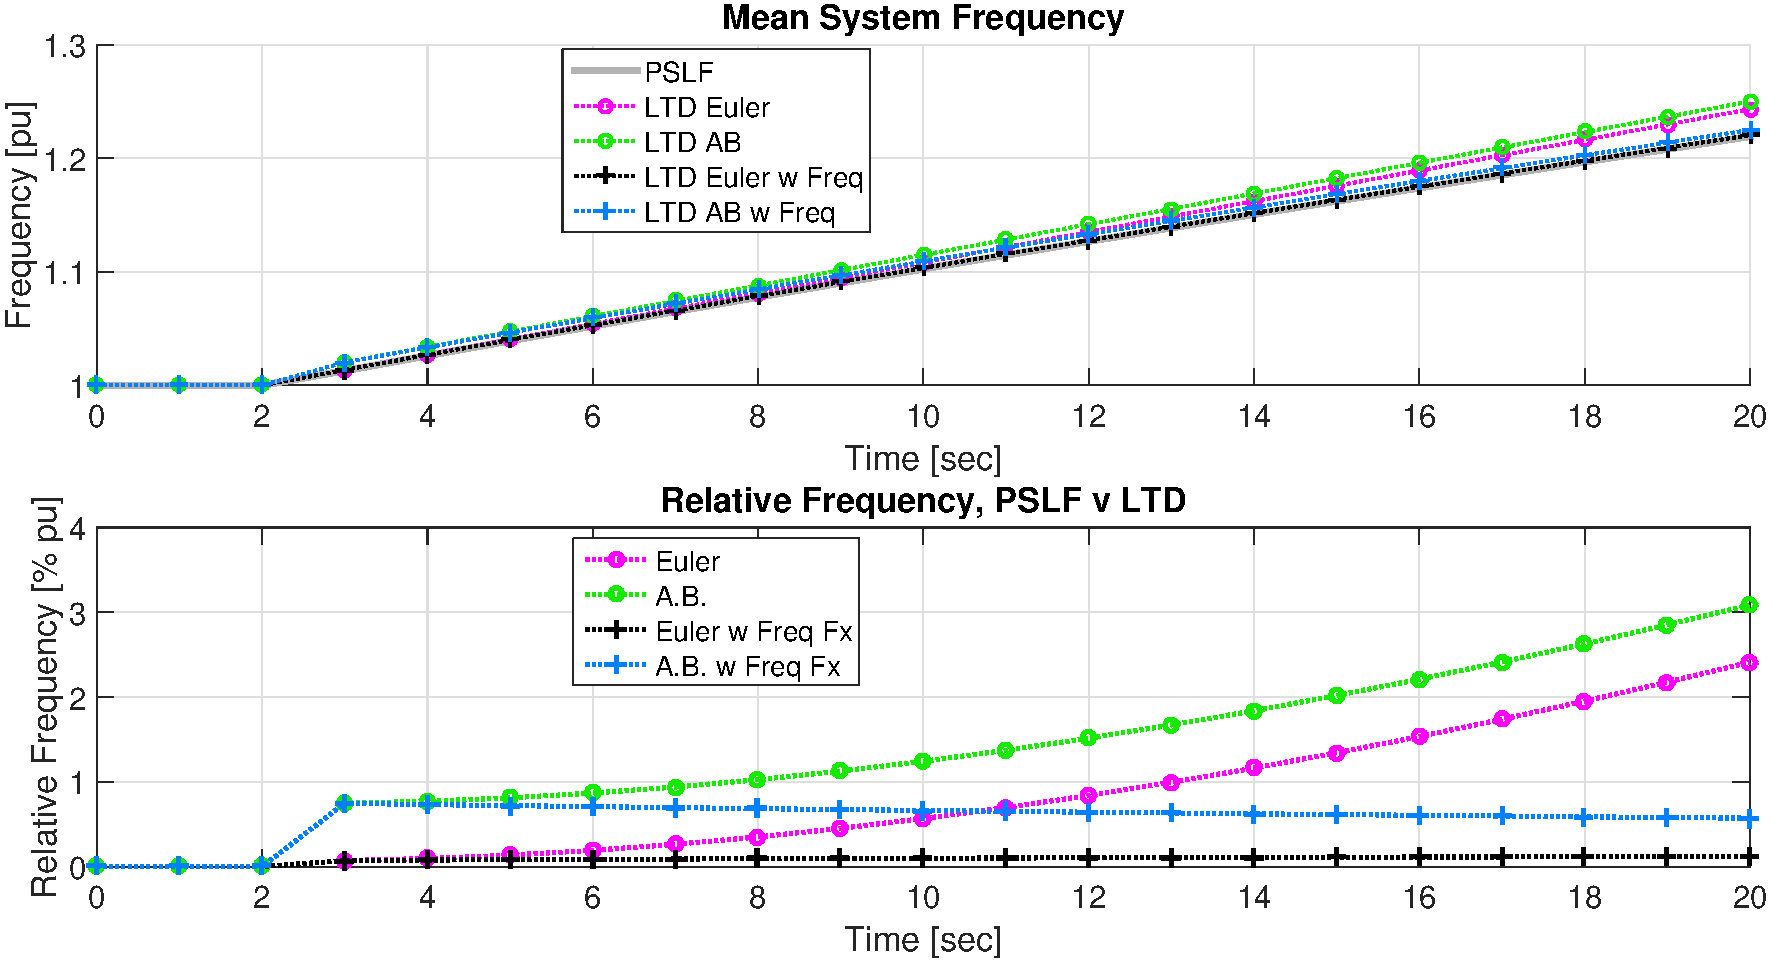
\includegraphics[width=\linewidth]{noGovExcLoadStepDfreq}
\end{figure}
\end{frame}

%************************************************
\section{Proof of Concept}
%________________________________________________
\subsection{Dynamic model 'pgov1' defined}
%------------------------------------------------
\begin{frame}[fragile]
pgov1 : Proportional gain control of $P_M$ \\

\begin{figure}
	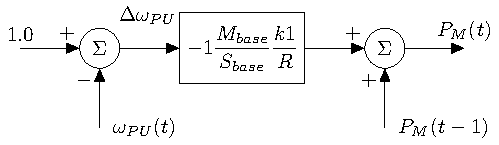
\includegraphics[width=\linewidth]{pgov1}
\end{figure}\vspace{-1em}
Entered into system via parsed text file:
\begin{lstlisting}[frame=single, basicstyle=\footnotesize]
# model  busnum busnam basekv id : #9 mwcap droop
#!pgov1   11 "11" 22.00 "1 " : #9 mwcap=100.0 0.05
\end{lstlisting}\vspace{-0.5em}
\footnotesize Model adapted from [3]
\end{frame}

%________________________________________________
\subsection{Dynamic model 'pgov1' experiment: +1 MW t=2, -1 MW t=30}
%------------------------------------------------
\begin{frame}
pgov1 on Gen 1, $t_\text{step}=$1.0 second
\begin{figure}
	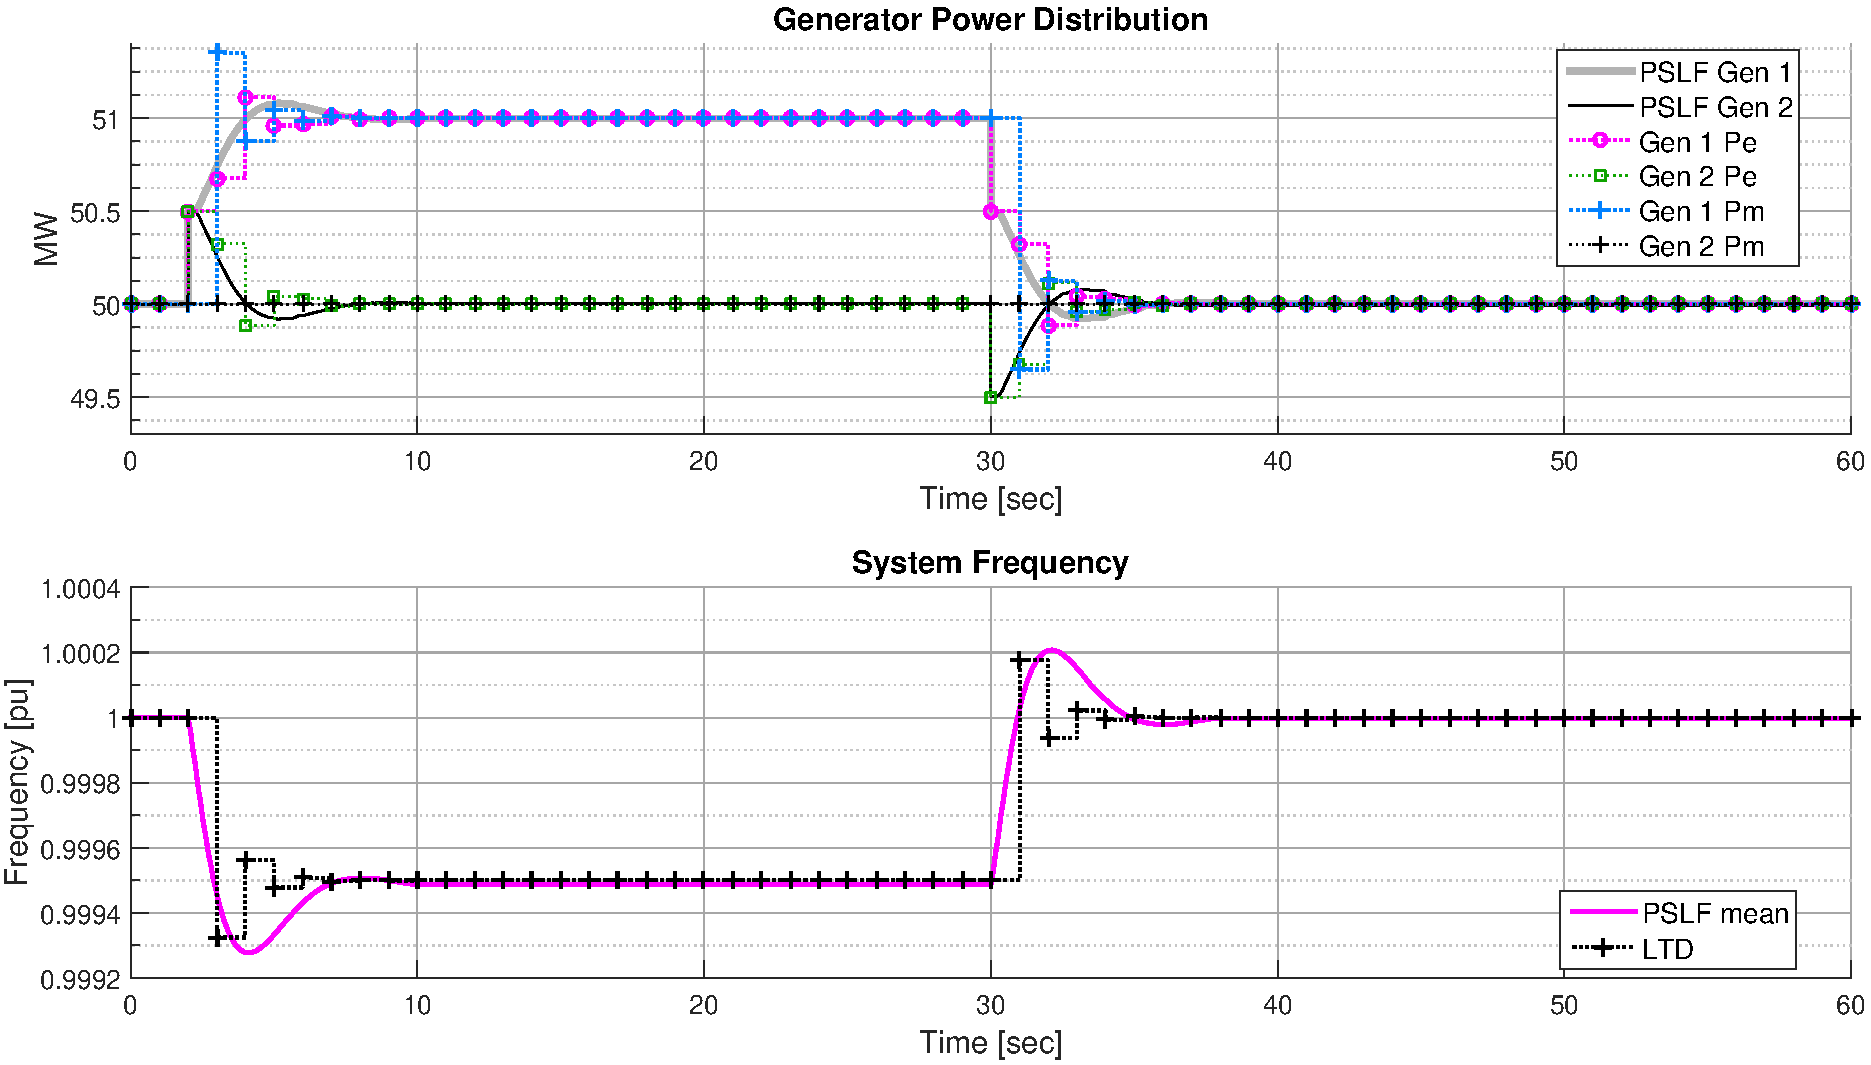
\includegraphics[width=\linewidth]{pgov1TestA}
\end{figure}
\end{frame}
%------------------------------------------------
\begin{frame}
pgov1 on Gen 1, $t_\text{step}=$0.5 second
\begin{figure}
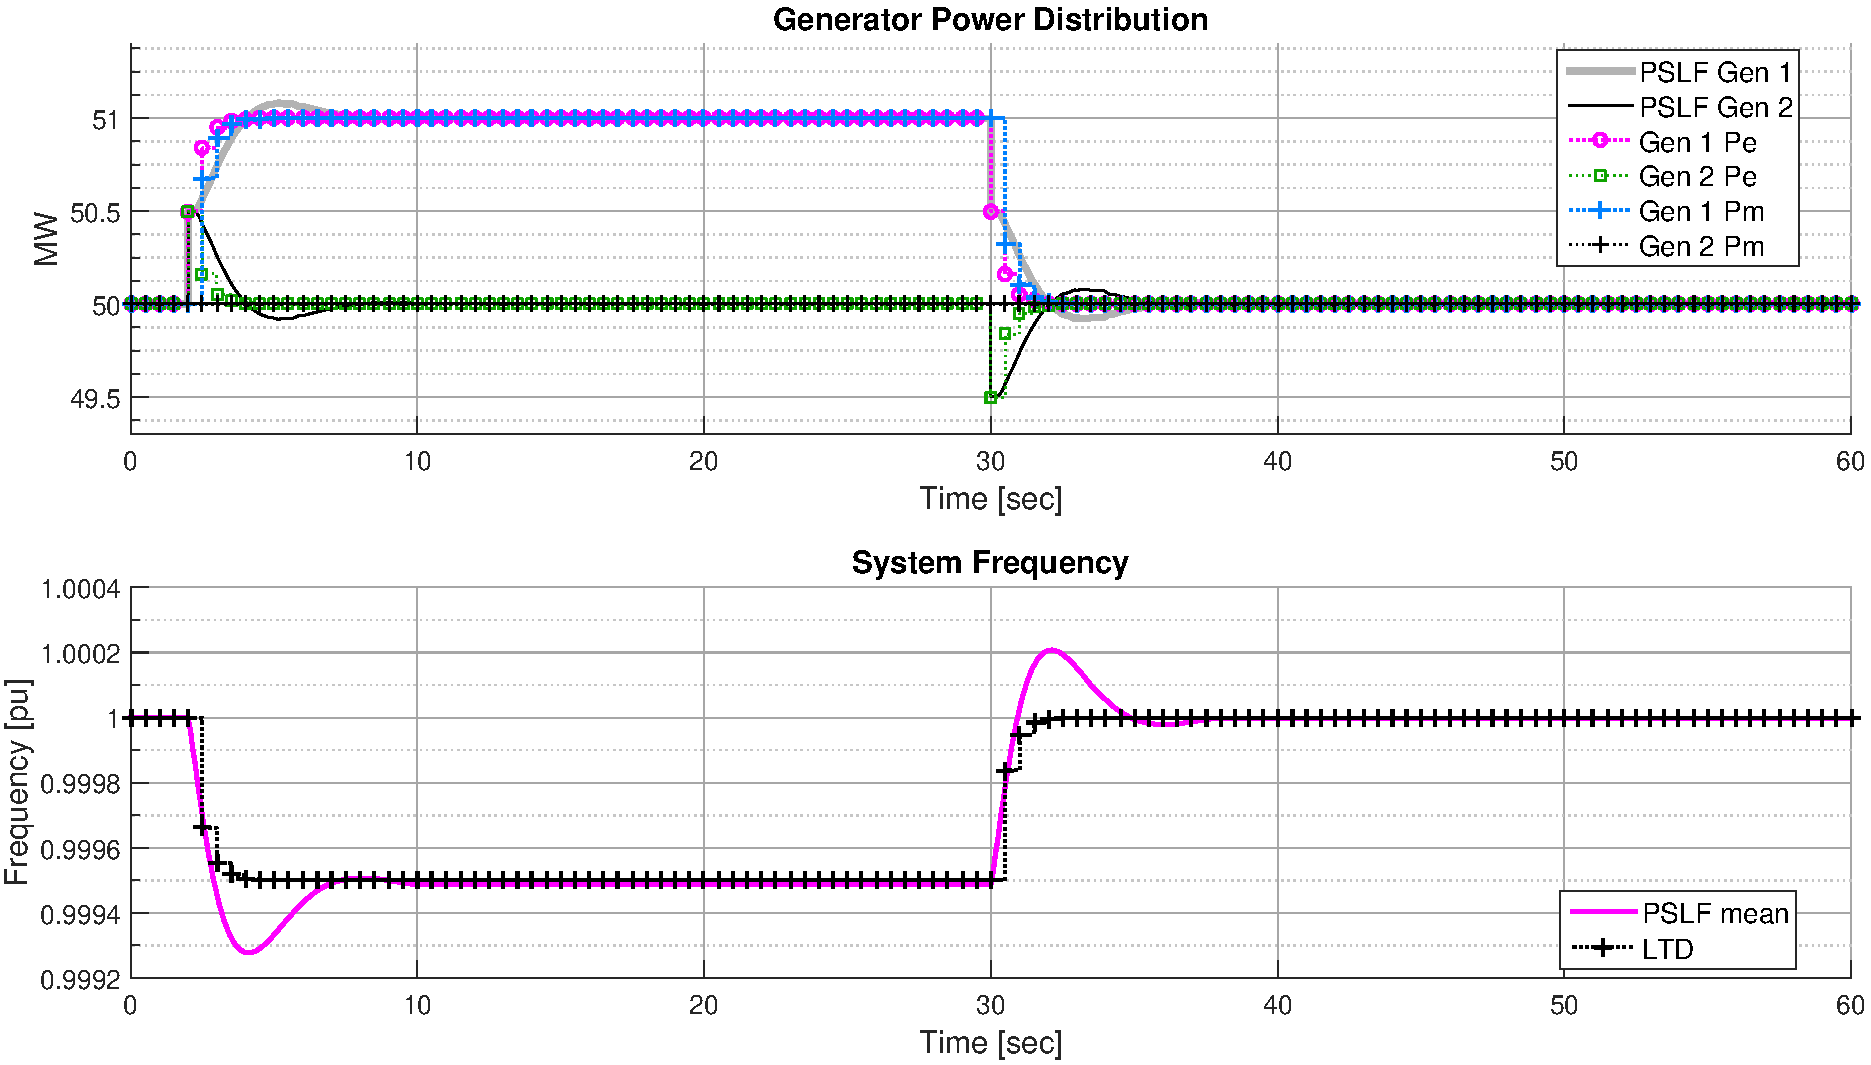
\includegraphics[width=\linewidth]{pgov1TestC}
\end{figure}
\end{frame}
%------------------------------------------------
\begin{frame}
pgov1 on Gen 1, $t_\text{step}=$0.5 second AB
\begin{figure}
	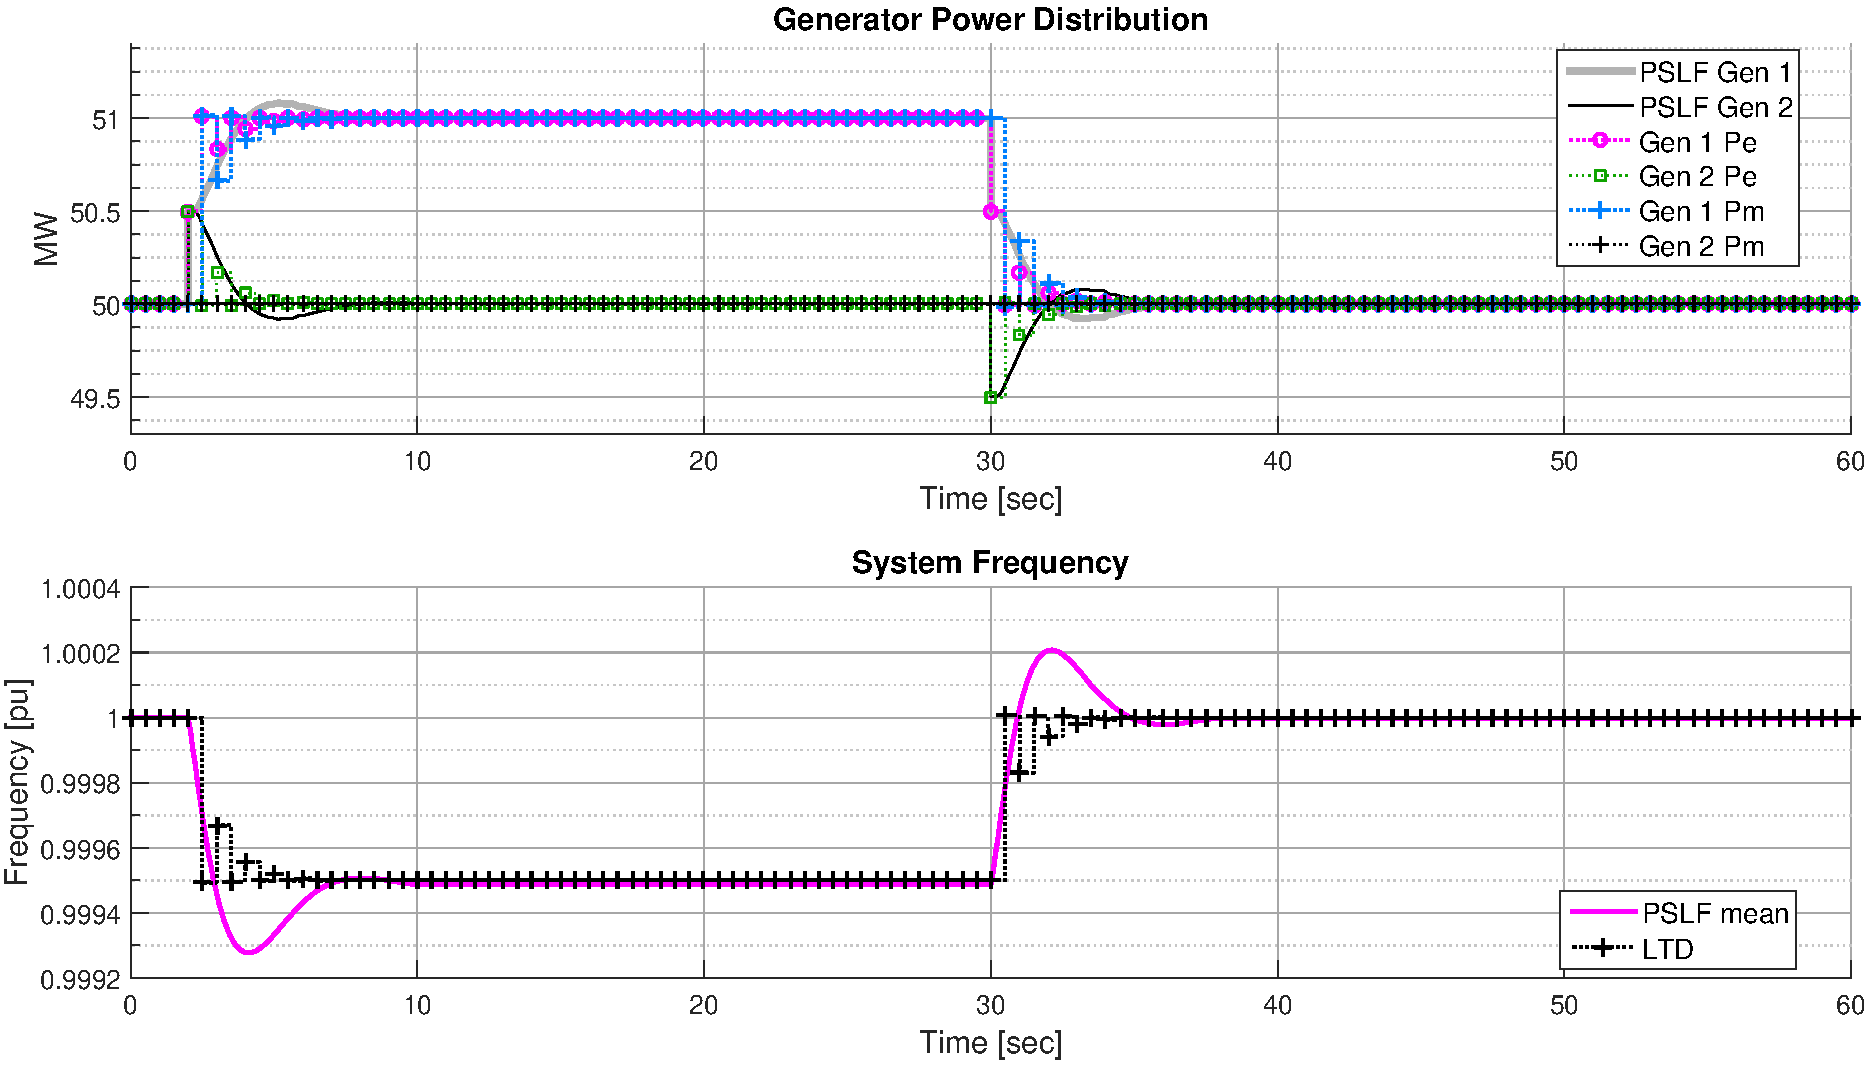
\includegraphics[width=\linewidth]{pgov1TestCab}
\end{figure}
\end{frame}

%------------------------------------------------
\begin{frame}
pgov1 on both Gens, $t_\text{step}=$0.5 second
\begin{figure}
	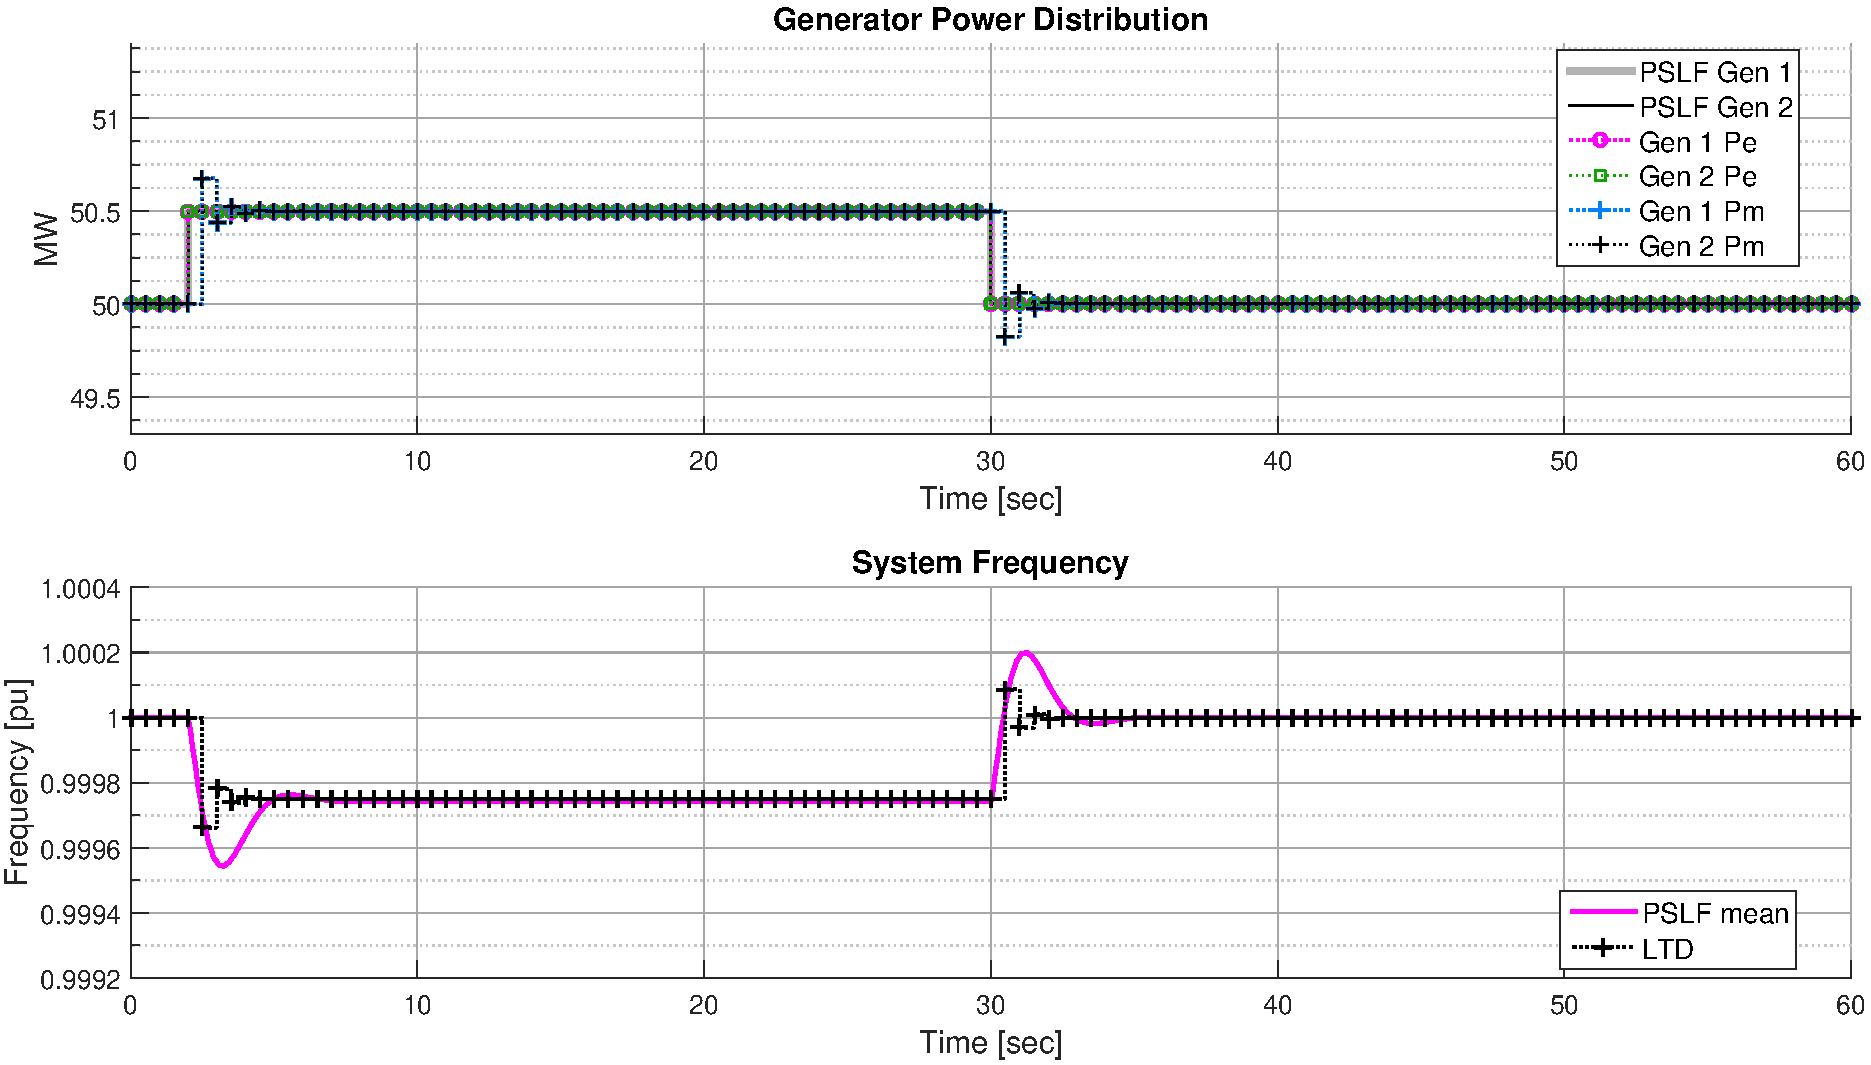
\includegraphics[width=\linewidth]{pgov1TestD}
\end{figure}
\end{frame}
%------------------------------------------------
\begin{frame}
pgov1 on both Gens, $t_\text{step}=$1 second
\begin{figure}
	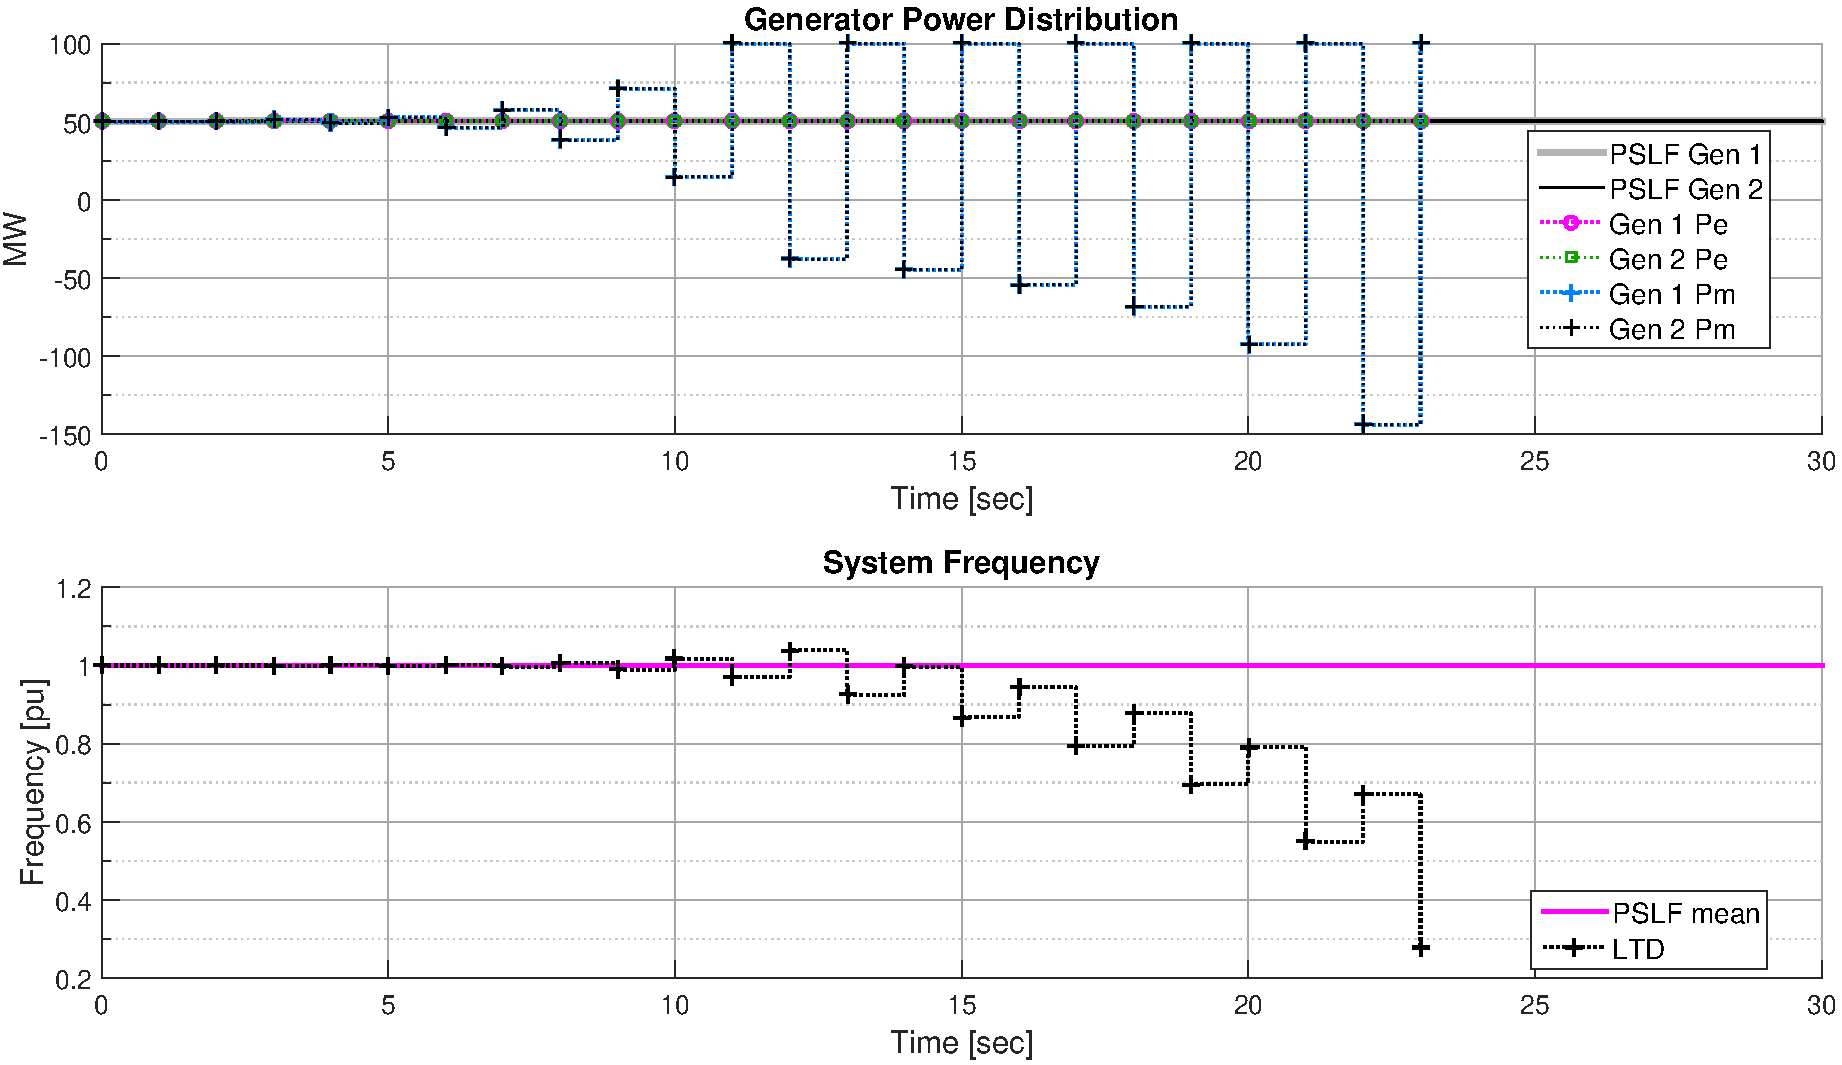
\includegraphics[width=\linewidth]{pgov1TestB}
\end{figure}
\end{frame}
%------------------------------------------------
\begin{frame}
Detail, $t_\text{step}=$1 second
\begin{figure}
	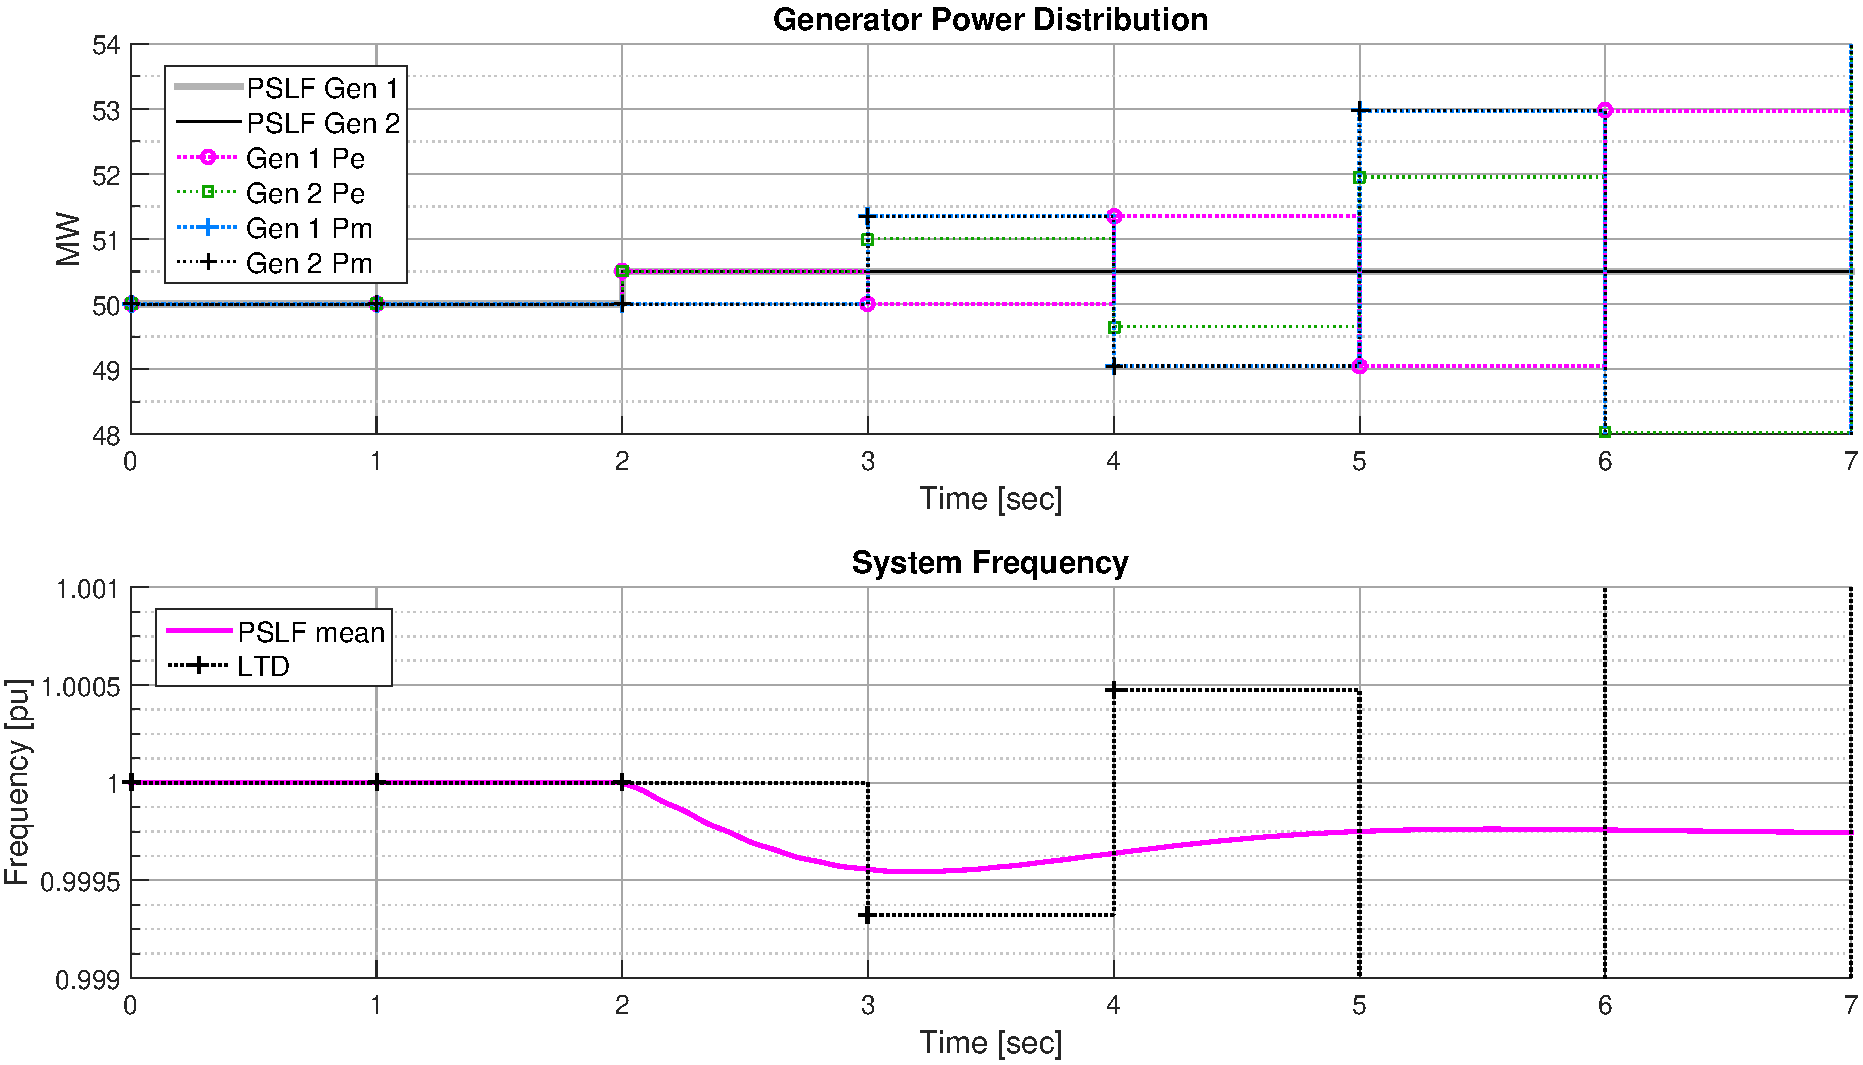
\includegraphics[width=\linewidth]{pgov1TestBdetail}
\end{figure}
\end{frame}

%************************************************
\section{Current Conclusions}
%------------------------------------------------
\begin{frame}
\begin{itemize}
	\item Much more work to do.
\end{itemize}
However,
\begin{itemize}
	\item Frequency effects should be accounted for in swing equation.
	\item Euler Integration tracks PSLF mean frequency well.
	\item Custom dynamic model implementation seems realizable. 
\end{itemize}
\end{frame}
%------------------------------------------------

\begin{frame}
References\vspace{1em}\\
%\resizebox{.8\textwidth}{.4\textheight}{
\begin{minipage}{\textwidth}
	\footnotesize
	\begin{itemize}
	\item[[1] GE Energy. "Mechanics of Running PSLF Dynamics" Phoenix, AZ, 2015
	\item[[2] Rand, W. (2018). Agent-Based Modeling: What is Agent-Based Modeling? [Online] Available: https://www.youtube.com/watch?v=FVmQbfsOkGc
	\item[[3] P.M. Anderson and A.A. Fouad, Power System Control and Stability, 2nd ed. IEEE Press, 2003, p20.
\end{itemize}
\end{minipage}
%}
\end{frame}
\end{document}